\chapter{Literaturübersicht}
\label{kap:literaturübersicht}
In der heutigen Zeit gibt es eine Vielzahl von Hilfsmitteln, um Zugverspätungen zu visualisieren. Ein bekanntes Hilfsmittel sind etwa das Live-Tracking von Zügen, wie es Tools wie Zugradar\footnote{\url{https://www.zugverfolgung.com/}} anbietet. Jedoch gibt es auch diverse Forschungsprojekte, welche sich der Visualisierung von Zugverspätungen widmen. Ein solches Projekt ist beispielsweise Trains of Data von SENSEable City Lab \parencite{trains_of_data_2012}. Als Teil des Trains of Data Projektes wurde die Visualisierung \textbf{Trains in Time} erstellt. Trains in Time ist eine Visualisierung des Zugnetzwerkes von Paris und betrachtet nebst den Verspätungen auch die Anzahl der Zugpassagiere (siehe Abbildung \ref{fig_trains_in_time}).

\begin{figure}[H]
    \caption{Trains in Time \parencite{trains_of_data_2012}}
    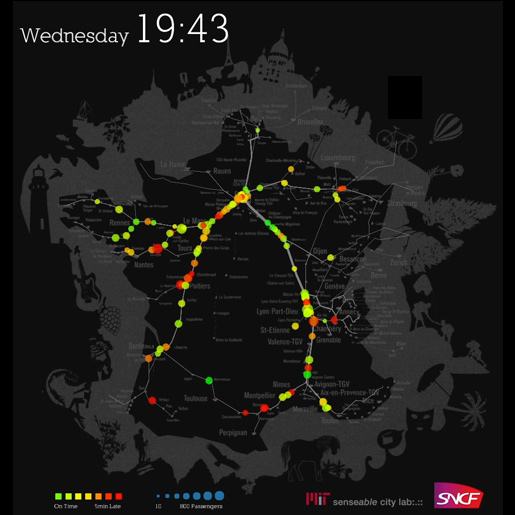
\includegraphics[height=10cm]{content/00_assets/trains_in_time.jpg}
    \label{fig_trains_in_time}
\end{figure}

Die nachfolgende Literaturübersicht soll einen Überblick über relevante Projekte und Visualisierungen schaffen, welche sich insbesondere mit Zugverspätungen und dessen Auswirkungen auseinandersetzen.
